\chapter{Simulated Annealing}
\section{Introduction}
The Simulated Annealing search algorithm is examined in this chapter, looking  initially at the strategy options and configuration choices. The results section shows the performance of the algorithm in preliminary trials with a range of annealing schedules before presenting the results of the main trials. 

\section{Search Strategy Options}
To be consistent with efforts of Random Search and Hill Climbing we again limit each trial to 25000 evaluations of the objective function. The operators used for Simulated Annealing are those that were used with Hill Climbing, however we have reduced the probability of occurrence of the shrink and grow operators based on our observations regarding duplication of solutions as discussed in Section~\ref{duplicate_solutions}.

The approach in general is similar to Hill Climbing, as the operators have been selected to allow fine-grained exploration of the search space while exploiting the capability of Simulated Annealing to avoid the pitfalls of local optima. The principle strategy choice for Simulated Annealing will be the selection of a suitable annealing schedule (see Section~\ref{schedule}), this is covered in detail in Section~\ref{schedule_selection}.



\section{Experimental Conditions}
Table~\ref{sa_param_table} shows the parameters used to configure Simulated Annealing. Symbolic Integration, Santa Fe and Blocks use initial Genome lengths of 100 while Symbolic Regression uses an initial length of 200. A temperature change rate of 0.95 is used to reduce the temperature on each iteration. A minimum temperature of \emph{0} is used to halt the annealing schedule. For a more complete explanation Section~\ref{sa_algorithm} provides a step-by-step guide to the algorithm.



\begin{table}[!hbp]
\begin{center}
\begin{tabular}{|l|l|l|l|l|}
\hline
Parameter &\multicolumn{4}{l|}{Problems}\\
\cline{2-1} \cline{3-1} \cline{4-1} \cline{5-1} 
 & Sym Int & Santa Fe & Blocks & Sym Reg  \\
\hline
Number of Trials & 1000 & 1000 & 1000 & 1000  \\
Number of Objective & & & & \\ 
Function Evaluations  & 25000 & 25000 & 25000 & 25000 \\
Initial Genome Length & 100 & 100 & 100 & 200  \\
Variation Range  & 10\% & 10\% & 10\% & 10\%  \\
Zero Improvement Accept  & off & off & off & off  \\
Probability of Selecting & & & & \\
Shrink Operator  & .05 & .05 & .05 & .05  \\
Probability of Selecting & & & & \\
Grow Operator  & .05 & .05 & .05 & .05  \\
Probability of Selecting & & & & \\
Force-up Operator  & .45 & .45 & .45 & .45  \\
Probability of Selecting & & & & \\
Force-down Operator  & .45 & .45 & .45 & .45 \\
Temperature Change Rate & 0.95 & 0.95 & 0.95 & 0.95  \\
Minimum Temperature & 0 & 0 & 0 & 0  \\
\hline
\end{tabular}
\caption{\label{sa_param_table} Parameters used for the Simulated Annealing Search Algorithm.}
\end{center}
\end{table}


\section{Establishing an Annealing Schedule}
\label{schedule_selection}The establishment of an appropriate annealing schedule for each of the problems centres on selecting the desired level of probability for acceptance of a dis-improving solution. 
At a temperature $t$, the probability $P$ for a change  in energy of magnitude $\delta E$ is given by 

\large
\begin{displaymath}
P(\delta E) = e ^{ \frac{-\delta E}{kt}}
\end{displaymath}
\normalsize

Figure~\ref{santafe_accept_prob_score_delta} shows the change in the probability of accepting a dis-improving solution for a range of score deltas. Three different temperatures have been shown. If it was possible to predict the type of score deltas we were likely to see in the course of a trial then we could usefully employ this information to select a suitable starting temperature. We know from the analysis of the Hill Climbing results that solutions often emerge from areas of the solution landscape where scores are low score. This might suggest that it is reasonable to accept large dis-improving deltas late in a trial. However this policy would also have the consequence of having us accept even larger score deltas early in a trial, this could force the search to remain trapped in sub optimal regions of the search space.

This is better illustrated in Figure~\ref{santafe_accept_prob_score_temp} which again shows the change in the probability of accepting a dis-improving solution but this time it has been plotted against increasing temperature. Three plots for score deltas of 1, 5 and 10 have been included. Again we see some of the trade offs in this graph a high starting temperature exposes the search to higher probabilities of moving into low scoring regions of the search space while starting with a very low temperatures might leave the search unable to effectively explore the search space because of a overly captious approach.


\begin{figure}[]
\centerline{\hbox{
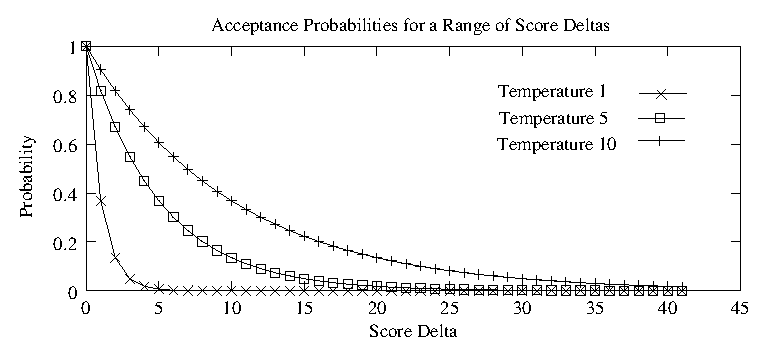
\psfig{file=Chapter7/graphs/accept_prob_score_delta.ps,width=4in}}}
\caption[Probability of accepting a dis-improving Solution for a Range of Score Deltas]{Probability of accepting a dis-improving Solution for a Range of Score Deltas at three different Temperatures on the Santafe Trail Problem.}
\label{santafe_accept_prob_score_delta}
\end{figure}


\begin{figure}[]
\centerline{\hbox{
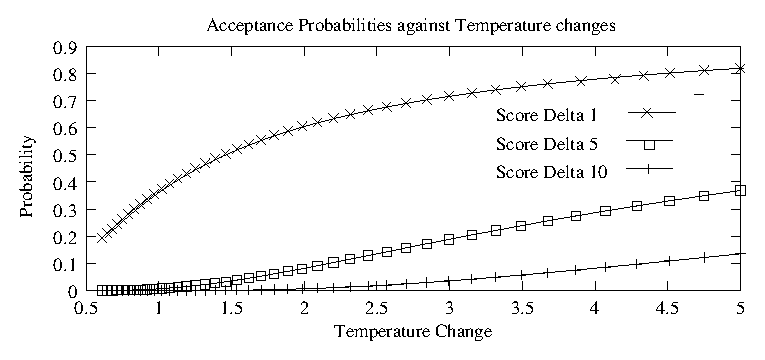
\psfig{file=Chapter7/graphs/accept_prob_temp_change.ps,width=4in}}}
\caption[Probability of accepting a dis-improving Solution for a Range of Temperatures]{Probability of accepting a dis-improving Solution for a Range of Temperatures at three different Score Deltas on the Santafe Trail Problem.}
\label{santafe_accept_prob_score_temp}
\end{figure}

In order to get some indication of suitable  annealing schedules for the problems a limited number of runs were first performed for a range of starting temperatures. The number of iterations at each temperature accordingly  varied in order to maintain our limit of 25000 evaluations of the objective function in a single trial.
The results of these preliminary runs plus the results of the extended runs are presented in the next section.



\section{Results}

Tables~\ref{sa_symint_sched_table},~\ref{sa_santafe_sched_table} and~\ref{sa_blocks_sched_table} show the results from the preliminary trials used to determine the appropriate annealing schedule for Symbolic Integration, Santa Fe and Blocks respectively. Similar runs on the Symbolic Regression problem failed to find any correct solutions. 

These preliminary trials consisted of 500 runs for each start temperature. The table shows the starting temperature and  the number of successes achieved.

For the case of Symbolic Integration the success rate appears to peak at 11\% for starting temperatures of 1 with the success rate trailing off either side of this. On the Santa Fe problem we see a plateau of similar scores for temperatures of 1 or less with a significant fall off in success rates for higher starting temperatures. The schedules for Blocks follows a  similar pattern to that of Santa Fe showing higher success rates at starting temperatures of one or less. The Symbolic Regression problem was not solved in any of the preliminary trials.


  
\begin{table}[h]
\begin{center}
\begin{tabular}{|l|l|}
\hline
Starting Temperature & Successful Runs \\
\hline
0.3 & 10\% \\
0.1 & 6\% \\
1   &  11\% \\
5   &  5\% \\
10  & 2\% \\
\hline
\end{tabular}
\caption{\label{sa_symint_sched_table} Results from 500 trials of Simulated Annealing on the Symbolic Integration Problem for a Range of Starting Temperatures.}
\end{center}
\end{table}



\begin{table}[h]
\begin{center}
\begin{tabular}{|l|l|}
\hline
Starting Temperature &  Successful Runs \\
\hline
0.3   &  17\%\\
0.1   &  20\%\\
1    &  19\% \\
5    &  4\% \\
10   &  5\% \\
\hline
\end{tabular}
\caption{\label{sa_santafe_sched_table} Results from 500 trials of Simulated Annealing on the Santa Fe Trail Problem for a Range of Starting Temperatures.}
\end{center}
\end{table}

\begin{table}[h]
\begin{center}
\begin{tabular}{|l|l|}
\hline
Starting Temperature &  Successful Runs \\
\hline
0.1   &   11\%\\
0.3    &   13\%\\
1     &   12\%\\
5     &   6\%\\
10    &   9\%\\
\hline
\end{tabular}
\caption{\label{sa_blocks_sched_table} Results from 500 trials of Simulated Annealing on the Blocks Problem for a Range of Starting Temperatures.}
\end{center}
\end{table}


Table~\ref{sa_results_table} provides a summary of the final results for Simulated Annealing. 1000 runs were performed using most successful starting temperature of 1 from the preliminary trials. Symbolic Regression was not solved in any of the attempts, however Symbolic Integration and Blocks have similar success rates scoring 11\% and 13\% respectively, while Santa Fe scores 21\%.
While the algorithm is more successful on the Symbolic Integration and Santa Fe problems than Hill Climbing, the overall results are still poor relative to those of Random Search. 

\begin{table}[h]
\begin{center}
\begin{tabular}{|l|l|}
\hline
Problem & Successful Runs \\
\hline
Symbolic Integration & 11\% \\
Santa Fe Trail & 21\% \\
Blocks & 13\% \\
Symbolic Regression & 0\% \\
Spirals & 0\% \\
\hline
\end{tabular}
\caption{ \label{sa_results_table} Results from the Simulated Annealing Trials.}
\end{center}
\end{table}





\section{Characteristics of Solutions found by Simulated Annealing}

Table~\ref{sa_results_analysis_table} shows details of the solutions found by Simulated Annealing, wrapping features prominently in Santa Fe and Blocks. The average solution length for Santa Fe is 58 codons of which 48 are expressed. Symbolic Integration has solutions with an average genome length of 76 of which only 19 are expressed. An aspect of the results from the Blocks problem is that the number of expressed codons was 91, which is considerably greater than the average number of codons in a solution at 54. This aspect of the Block's results is caused by multiple wrap events where the codons are repeatedly re-used until a successful solution is found.  


\begin{table}[h]
\begin{center}
\begin{tabular}{|l|l|l|l|l|}
\hline
Feature & Sym Int & Santa Fe & Blocks & Sym Reg  \\
\hline
Avg Number of Codons & & & &  \\ 
in Solution & 76 & 58 & 54 & n/a  \\
Avg Number of expressed & & & &  \\
Codons in Solution & 19 & 48 & 91 & n/a  \\
Avg Number of Solutions & & & &  \\
featuring Wrapping & 0\% & 50\% & 66\% & n/a  \\
\hline
\end{tabular}
\caption{\label{sa_results_analysis_table} Analysis of Characteristics from Solutions found by Simulated Annealing.}
\end{center}
\end{table}




\subsection{Analysis of search trajectory}

A typical search trajectory for a Simulated Annealing trial is shown in ~\ref{sa_search1}. In the early stages the algorithm explores areas of both low and high fitness but as the trials progresses we see a steady climb to areas of high fitness as the decreasing temperature reduces the probability of selecting dis-improving solutions.

\begin{figure}[hbp]
\centerline{\hbox{
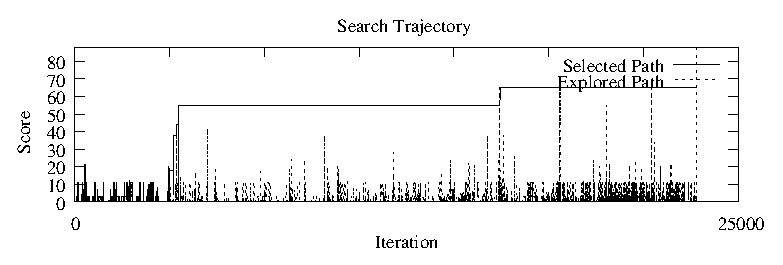
\psfig{file=Chapter7/graphs/search_trajectory_sa.ps,width=5in}}}
\caption{\label{sa_search1}Search Trajectory for a Successful Simulated Annealing Trial}
\end{figure}



\section{Summary}
In this chapter we have looked at Simulated Annealing, a metaheuristic, which models itself on the way crystals form in solids during the cooling process. The principle strategy choice for the method was the selection of a suitable annealing schedule, to assist this selection a number of preliminary trials were performed using a range of starting temperatures. The final results showed unsuccessful attempts on two of the problem, Symbolic Regression and Spirals and low success rates on the other three.

The additional capability of Simulated Annealing to avoid sub-optima would appear to have added little or no improvement on the scores achieved by Hill Climbing, leaving it a considerable way behind Random Search. 





















